\chapter{Introduction to quantum geometry}
\label{chap:driving}
This chapter heavily depends on the mathematical formalism developed in Chapter \ref{chap:mathIntro} and some basic knowledge of quantum mechanics is required.

Most parts of this chapter are inspired by \citet{kolodrubez} and original notes by \citet{berry1984}, \citet{berry1989}, \citet{berry2009} with attempt to give them more rigorous meaning in the language of differential geometry. We will see, that the structure of the space on which the quantum state driving will be performed is quite complicated. The reason is that it has a fiber structure, where every fiber is another fiber bundle. Luckily what we will use later on are sections of this space, which will be much easier Riemannian manifolds. 

There may be many geometrical constructions of the space, because usually only some special sections of the full space are used. Different constructions require different mathematical formalism. One might choose the way of \emph{vector bundles}, or \emph{fiber bundles} (our case), or just sectioning one Hilbert space in different ways, constructing the needed physical spaces. The reason for choosing the way of fiber bundles is that from the Hamiltonian with free parameter $\HH(\lambda)$ we get one Hilbert space for every value of the parameter. The fiber structure then gives the natural formalism for connecting these spaces.

The theory constructed below strongly depends on differential geometry, but it does not reformulate the whole quantum mechanics into this language. This is rather complicated task and for basics of this theory, see Appendix \ref{appendixGEOM}.

From now on we will use natural units, so $\hbar=1$.

\section{Space of all states}
Assume parameter $\llambda\in\mathcal{U}\subset\R^d$ for $\mathcal U$ open set. This parameter controls some finite-dimensional Hamiltonian $\HH(\llambda)$, which is bounded from below and has discrete spectrum. From this we can construct the fiber bundle, such that at every point of the base manifold $\llambda\in \mathcal{U}$, we construct fiber as a Hilbert space $\H(\llambda)$. The fiber structure can be according to Def. \ref{def:fiberBundle} written as
$$\left(\H_{full}\coloneqq \bigcup_{\llambda\in\mathcal U} \H(\llambda),\;\;\mathcal{U}\subset \R^d,\;\;\pi,\;\; \H(\llambda) \coloneqq \bigcup_{states}\ket{\psi(\llambda)}  \right).$$
The projection is defined as $\pi(\llambda): \ket{\psi(\llambda)}\mapsto \llambda$ and $\H(\llambda)$ is a Hilbert space containing all pure states of $\HH(\llambda)$.  Geometric intuition is displayed in Fig. \ref{fig:wholeBundle}.

\begin{figure}[H]
    \centering
    % 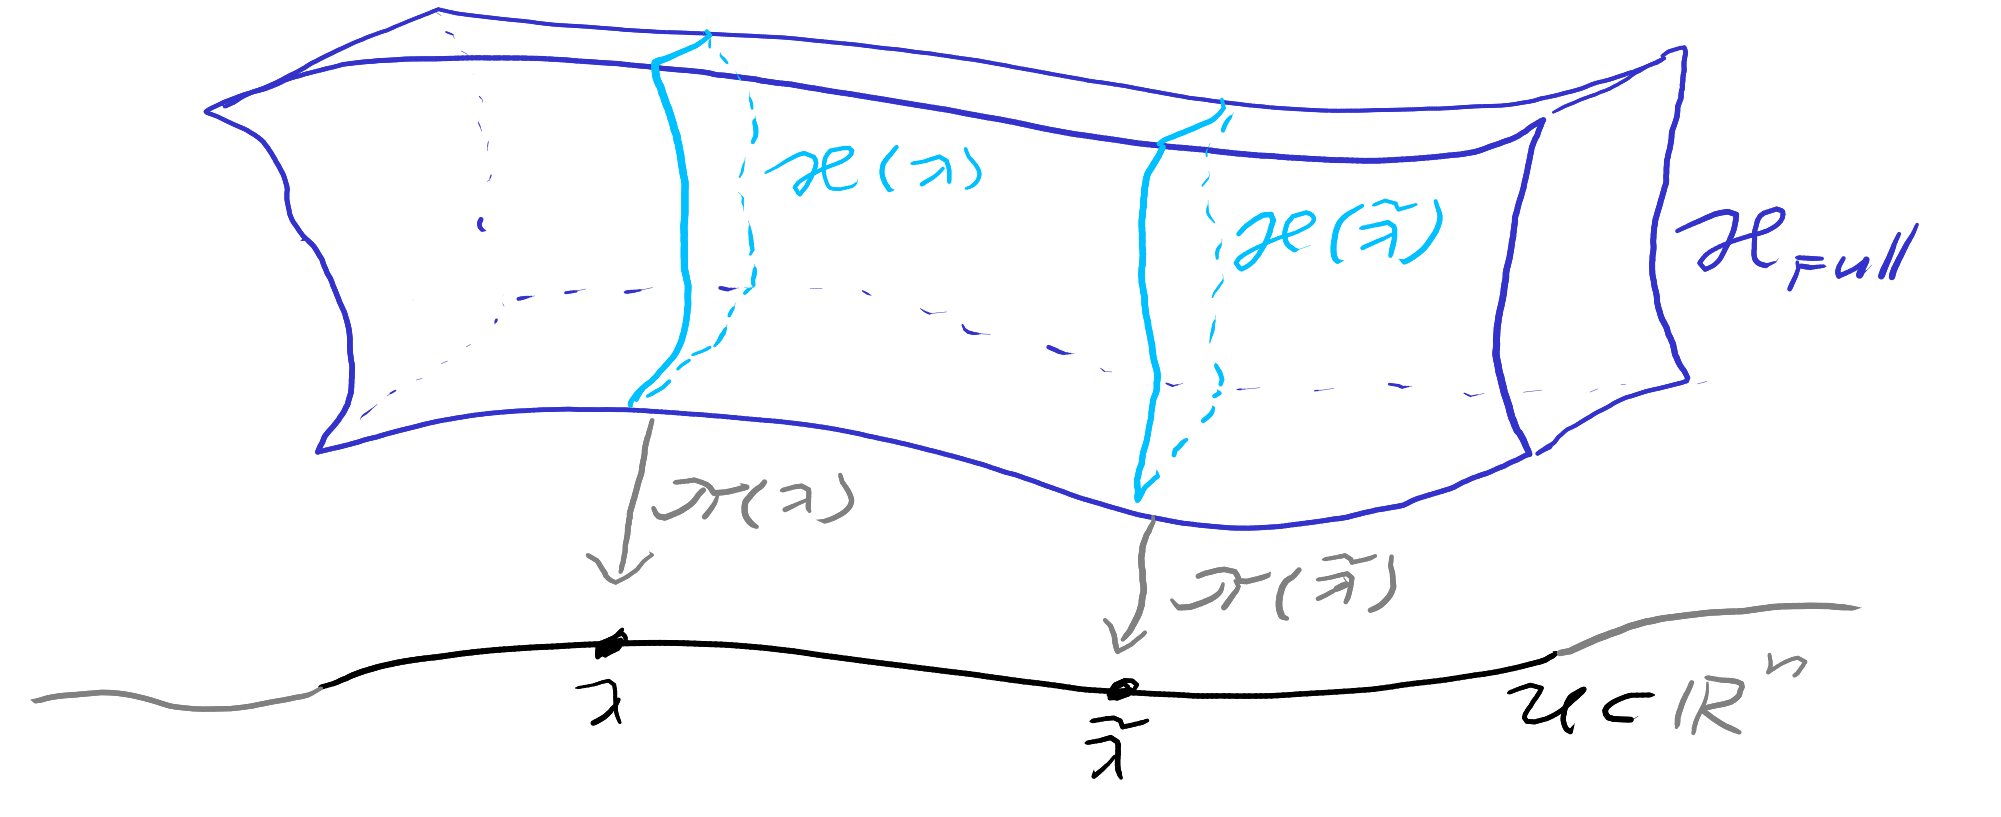
\includegraphics[width=\textwidth]{../img/manifold_basic_1.png}
    \begin{tikzpicture}
        \node[] at (0,0) {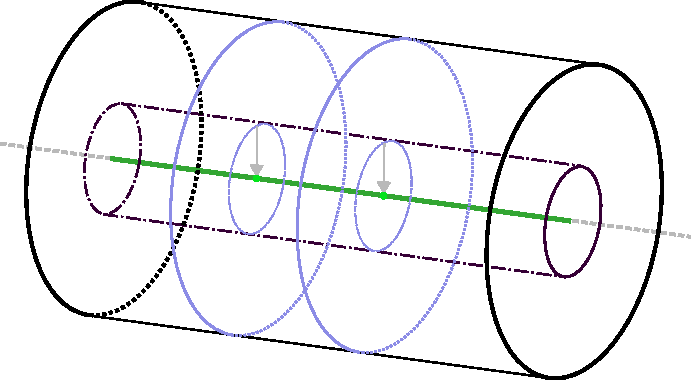
\includegraphics[width=0.7\textwidth]{../img/fullHilbert.pdf}};
        \node[] at (5.8,-0.7) {$\mathcal U\subset \gray{\R^n}$};
        \node[] at (4.6,1.8) {$\H_{full}$};
        \node[] at (-1.0,2.7) {$\blueee{\H(\llambda)}$};
        \node[] at (1.0,2.5) {$\blueee{\H(\tilde\llambda)}$};
        \node[] at (-0.8,0.55) {$\gray{\pi(\llambda)}$};
        \node[] at (1.05,0.3) {$\gray{\pi(\tilde\llambda)}$};
        \node[] at (-1.4,-0.17) {$\llambda$};
        \node[] at (0.5,-0.4) {$\tilde\llambda$};
    \end{tikzpicture}

\caption{Base manifold $\mathcal U\subset \R^d$ is visualized as a line. From every point $\llambda$ one Hilbert space $\H(\llambda)$ is constructed as a fiber. The union of all these fibers is full Hilbert space $\H_{full}$.}
    \label{fig:wholeBundle}
\end{figure}



\section{Rays and bare states}
In quantum mechanics, physical observables are related to the \emph{space of rays}, defined as $\P\H\coloneqq \H/U(1)$, where elements of $U(1)$ are unitary transformations $e^{i\varphi}$ for $\varphi\in\R$. This defines the \bluee{global} gauge symmetry between quantum states. The phase $\varphi$ is \bluee{chosen the same for every vector} and can be chosen arbitrarily. We cannot alter the phase of individual vectors, meaning there is no local gauge symmetry. The geometrical intuition is drawn on Fig. \ref{fig:projectiveHilbertSpace}.
\begin{figure}[H]
    \centering
    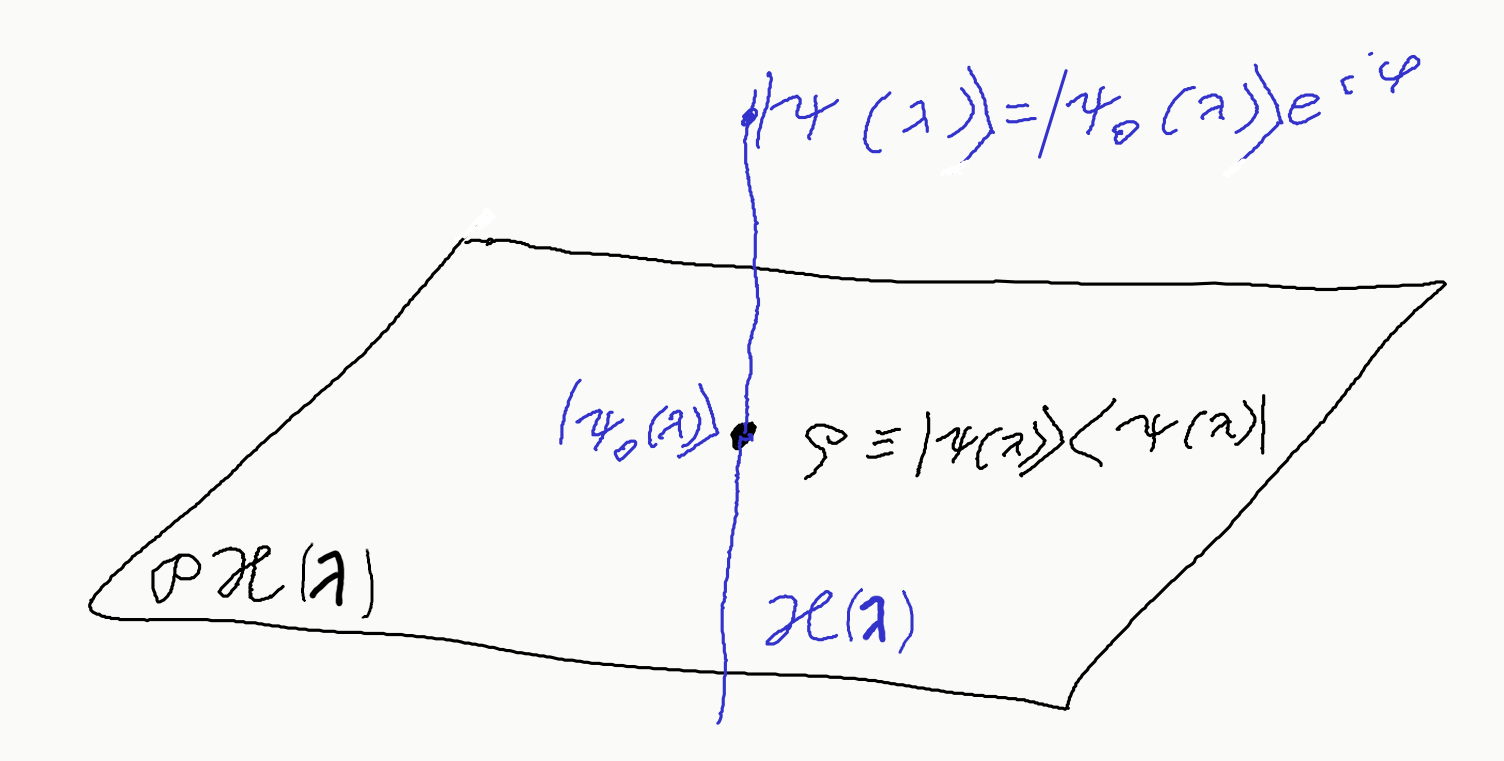
\includegraphics[width=0.8\textwidth]{../img/projectiveHilbertSpace.png}
\caption{For every $\llambda$ we have the Hilbert space $\H(\llambda)$ containing all states $e^{i\varphi}\ket{\psi(\llambda)}$. Global choice for the phase $\varphi$ fixes some projective Hilbert space $\P\H$. \red{draw it to ressemble the pictures above}}
    \label{fig:projectiveHilbertSpace}
\end{figure}

This resembles the fiber structure
$$\left(\H,\;\P\H,\;\pi_{rays},\;\{e^{i\varphi}| \varphi\in[0,2\pi)\}\right),$$
where $\pi_{rays}$ is just rule setting phase $\varphi$ to arbitrary value, which we will fix to $\varphi=0$.







\section{Sectioning the space}
Assume one begins with the state $\ket{\psi_0}$. The state then evolves along some path $\gamma\coloneqq\{\llambda(t)|t\in(0,T)\}\subset \mathcal U \subset \R^n$ parametrized by time, for which the Schr\"odinger equation
\begin{equation}
    i\hbar \der{}{t}\kpsilt = \HH(\llambda)\kpsilt
    \label{eq:schrodinger}
\end{equation}
holds. For eigenstates of instantaneous Hamiltonian it reads as a Schr\"odinger energy equation
\begin{equation}
    \HH(\llambda)\ket{s(\llambda)}=E_s(\llambda)\ket{s(\llambda)}.
    \label{eq:energySchrodinger}
\end{equation}
Notice that these states are independent on the trajectory $\gamma_t$.
For every $\HH(\llambda)$ its energies can be sorted from the smallest, defining the set 
\begin{equation}
    \sigma(\HH(\llambda))\coloneqq\{E_0,\dots,E_{n-1}\},
\end{equation}
which is called a \emph{Hamiltonian spectrum}. In this set, degeneracies are not unified into one element, therefore every $\sigma(\llambda)$ has $n$ elements. From this there exists an isomorphism between all $\sigma$-sets, and we can define \emph{section} 
$$\mathrm{sec}_s: \ket{s(\llambda)}\mapsto \mathcal{U}\subset \R^d, \quad \text{for } s\in\{0,\dots, n-1\}.$$
This maps eigenstates corresponding to energy $E_s$ to the base manifold. This mapping is similar to previously introduced $\pi$, except it is an isomorphism, not a projection. The isomorphism will be showed later on, when introducing the metric structure on these spaces.

Now we have constructed $n$ sections of the full Hilbert space, which are isomorphic to the base manifold. Because $\mathcal U$ is a Riemannian manifold, these so-called \emph{projective state manifolds} $\P\M_s$, must be also Riemannian.
Of special importance is the \emph{projective ground state manifold} $\P\M_0$, which will be used later on for adiabatic transports of ground states. Geometrical intuition is drawn on Fig. \ref{fig:fullStructure}. 

The reason for calling these manifolds \emph{projective} is the gauge symmetry of the Schr\"odinger equation. We can change the phase of vector $\kpsi\mapsto e^{i\varphi}\kpsi$ by any $\varphi$. Unifying over all phases, we get \emph{energy manifolds}
\begin{equation}
    \M_s\coloneqq \left\{\bigcup_{\varphi\in[0,2\pi)} \bigcup_{\llambda\in\mathcal U} e^{i\varphi}\ket{\psi(\llambda)}\right\}
\end{equation}

Because these manifolds were created by sectioning, they are considered to be vector spaces in a geometrical sense. This was expected, because they contain quantum states, which themselves are vectors.

\begin{figure}[H]
    \centering
    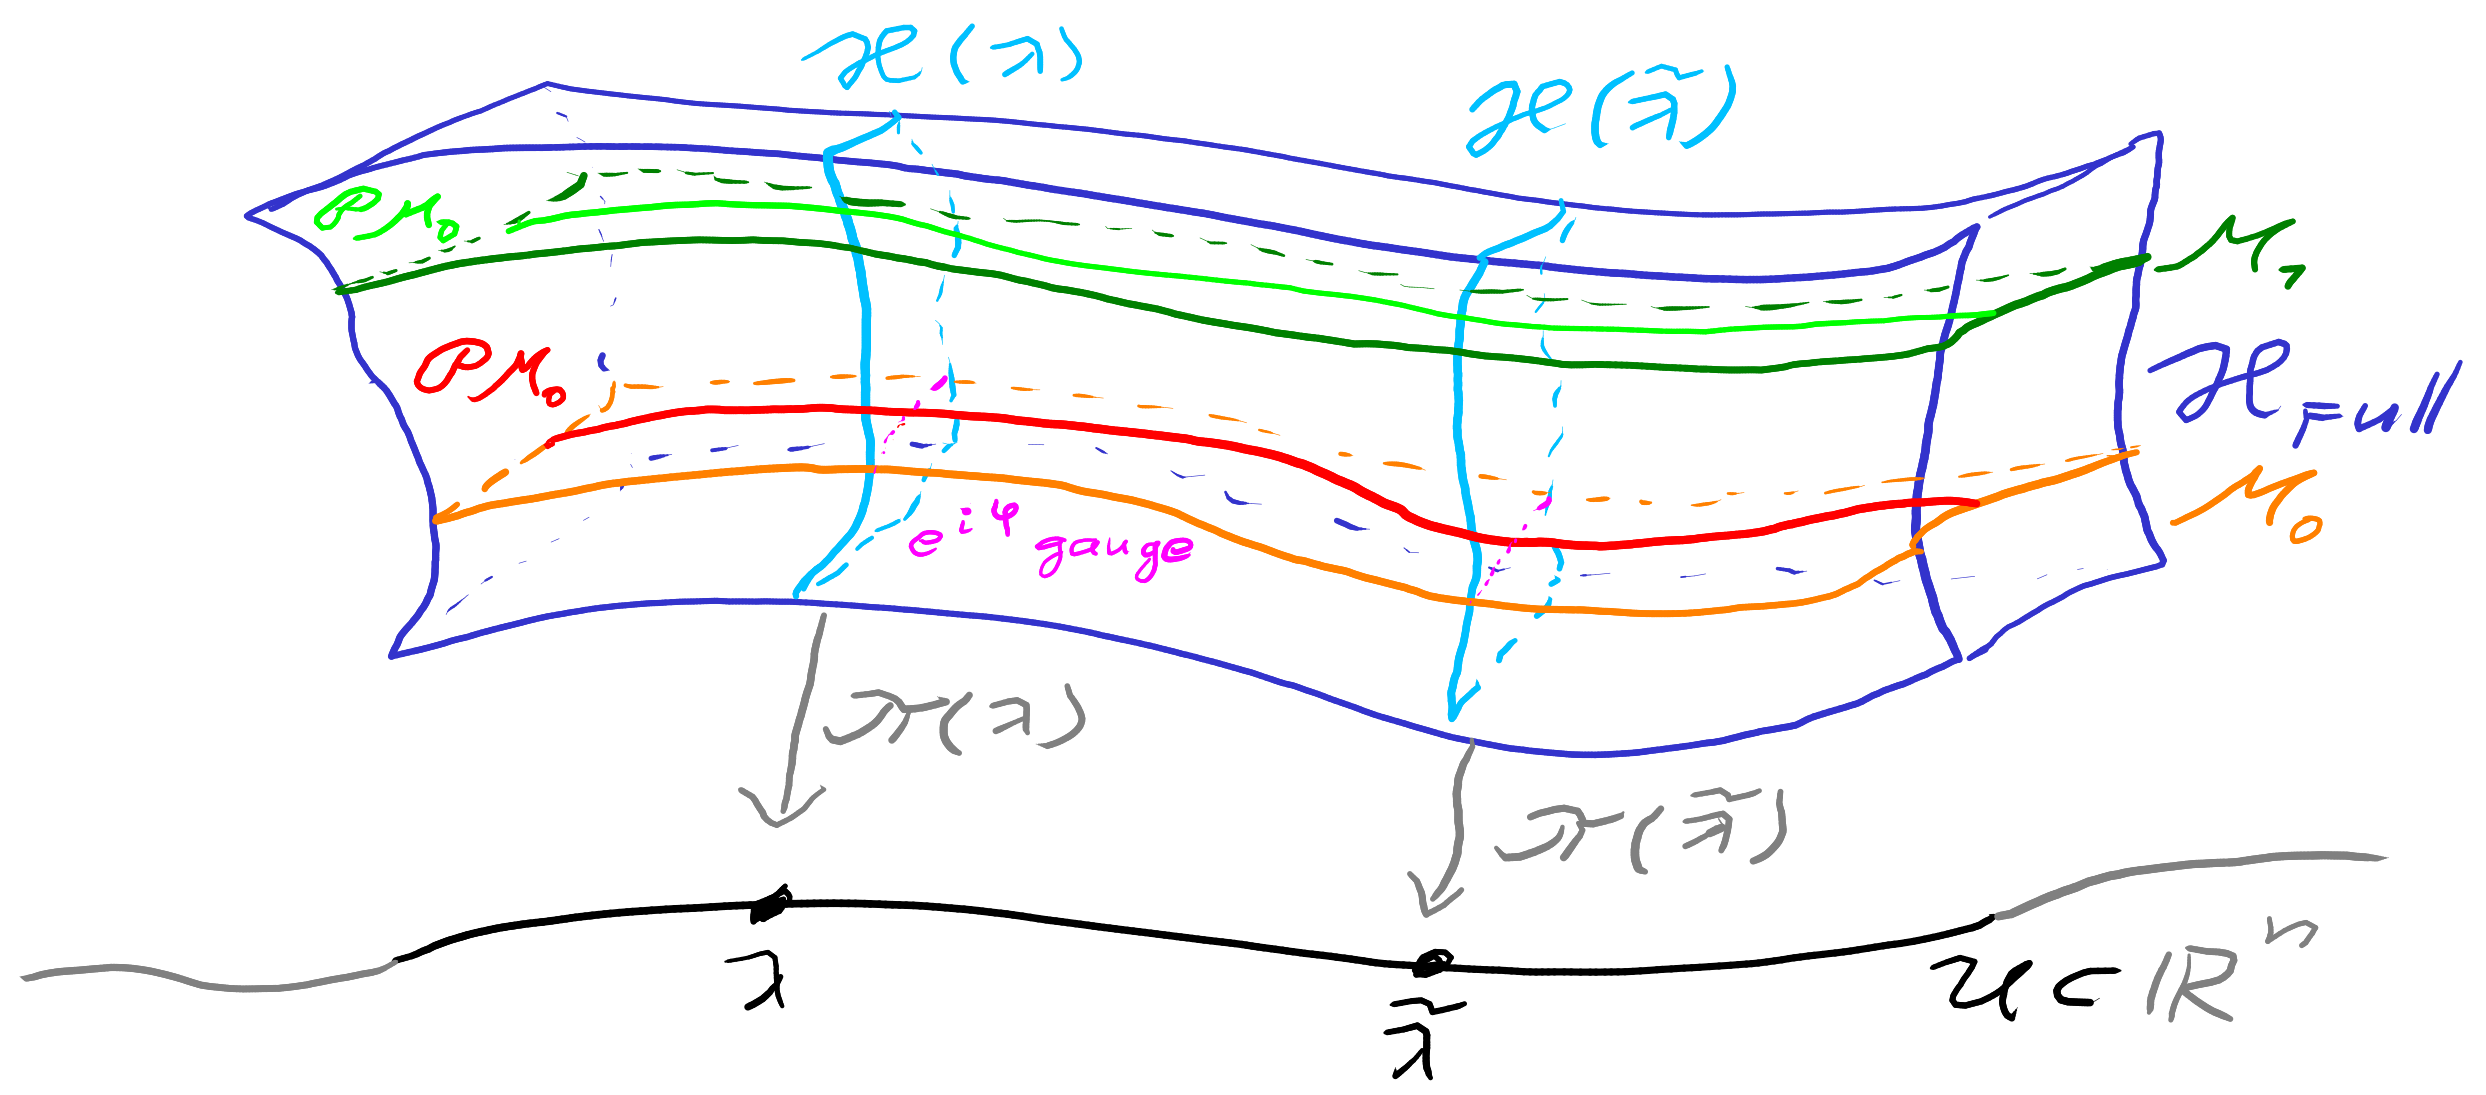
\includegraphics[width=\textwidth]{../img/manifold_full_1.png}
    \begin{tikzpicture}
        \node[] at (0,0) {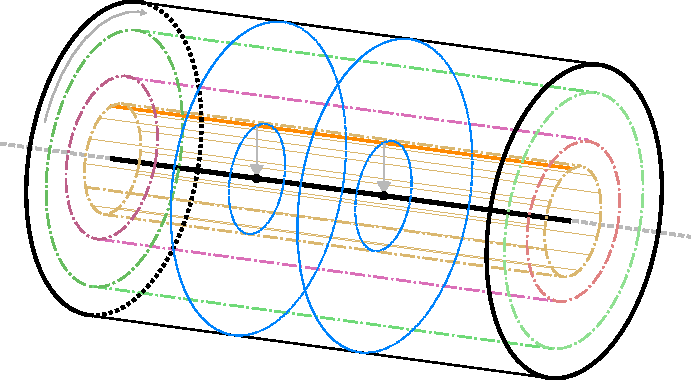
\includegraphics[width=0.7\textwidth]{../img/fullHilbert_1.pdf}};
        \node[] at (5.8,-0.7) {$\mathcal U\subset \gray{\R^n}$};
        \node[] at (4.6,1.8) {$\H_{full}$};
        \node[] at (-1.0,2.7) {$\blueee{\H(\llambda)}$};
        \node[] at (1.0,2.5) {$\blueee{\H(\tilde\llambda)}$};
        \node[] at (-0.8,0.55) {$\gray{\pi(\llambda)}$};
        \node[] at (1.05,0.3) {$\gray{\pi(\tilde\llambda)}$};
        \node[] at (-1.4,-0.17) {$\llambda$};
        \node[] at (0.5,-0.4) {$\tilde\llambda$};
        \node[] at (-4.1,1.0) {$\textcolor{orange}{\P\M_0}$};
        \node[] at (4.1,0.0) {$\textcolor{orange}{\M_0}$};
        \node[] at (4.15,0.5) {$\textcolor{violet}{\M_1}$};
        \node[] at (4.2,1) {$\textcolor{purple}{\M_s}$};
        \node[] at (-5.1,2.3) {$\gray{\varphi\in[0,2\pi)}$};
    \end{tikzpicture}
\caption{From the full Hilbert space we identified eigenstates. First was caused by the fiber structure and separates different \bluee{Hilbert spaces $\H(\llambda)$}. Newly introduced sectioning correspond to eigenstates of individual Hamiltonians and creates \greenn{Riemannian manifolds $\M_s$}. The phase \textcolor{violet}{$\varphi$} is drawn as another \textcolor{violet}{direction}.}
    \label{fig:fullStructure}
\end{figure}




The Hilbert spaces in different points $\llambda$ have the same finite dimension, so the natural question is if we really need the fiber structure and if we could understand the projection $\pi$ as a surjection from one Hilbert space to the base manifold $\pi: \H\rightarrow \M$. This can surely be done, but we would lose some generality. For example, the natural choice for basis in the Hilbert space is the eigenbasis. This basis is different for every $\H(\llambda)$ and this opens up two different approaches to a wave-function collapse.
\begin{enumerate}
    \item In the fiber structure, we can imagine changing the parameter $\llambda$ (so-called driving) as moving between $\H(\llambda)$ subspaces of $\H_{full}$, in which the eigenbasis can be embedded geometrically. The space structure can be precalculated, and every driving can be performed in this space.
    \item If we imagine only one Hilbert space, the eigenbasis varies in time and the driving is performed in a changing space in time.
\end{enumerate}








\section{Transporting states on state manifolds}
This chapter is inspired by \citet{berry1984}. We will decompose of $\H_{full}$ to different state manifolds $\M_s$, as displayed on figure \ref{fig:manifoldCutIntuition}.

\begin{figure}[h]
    \centering
    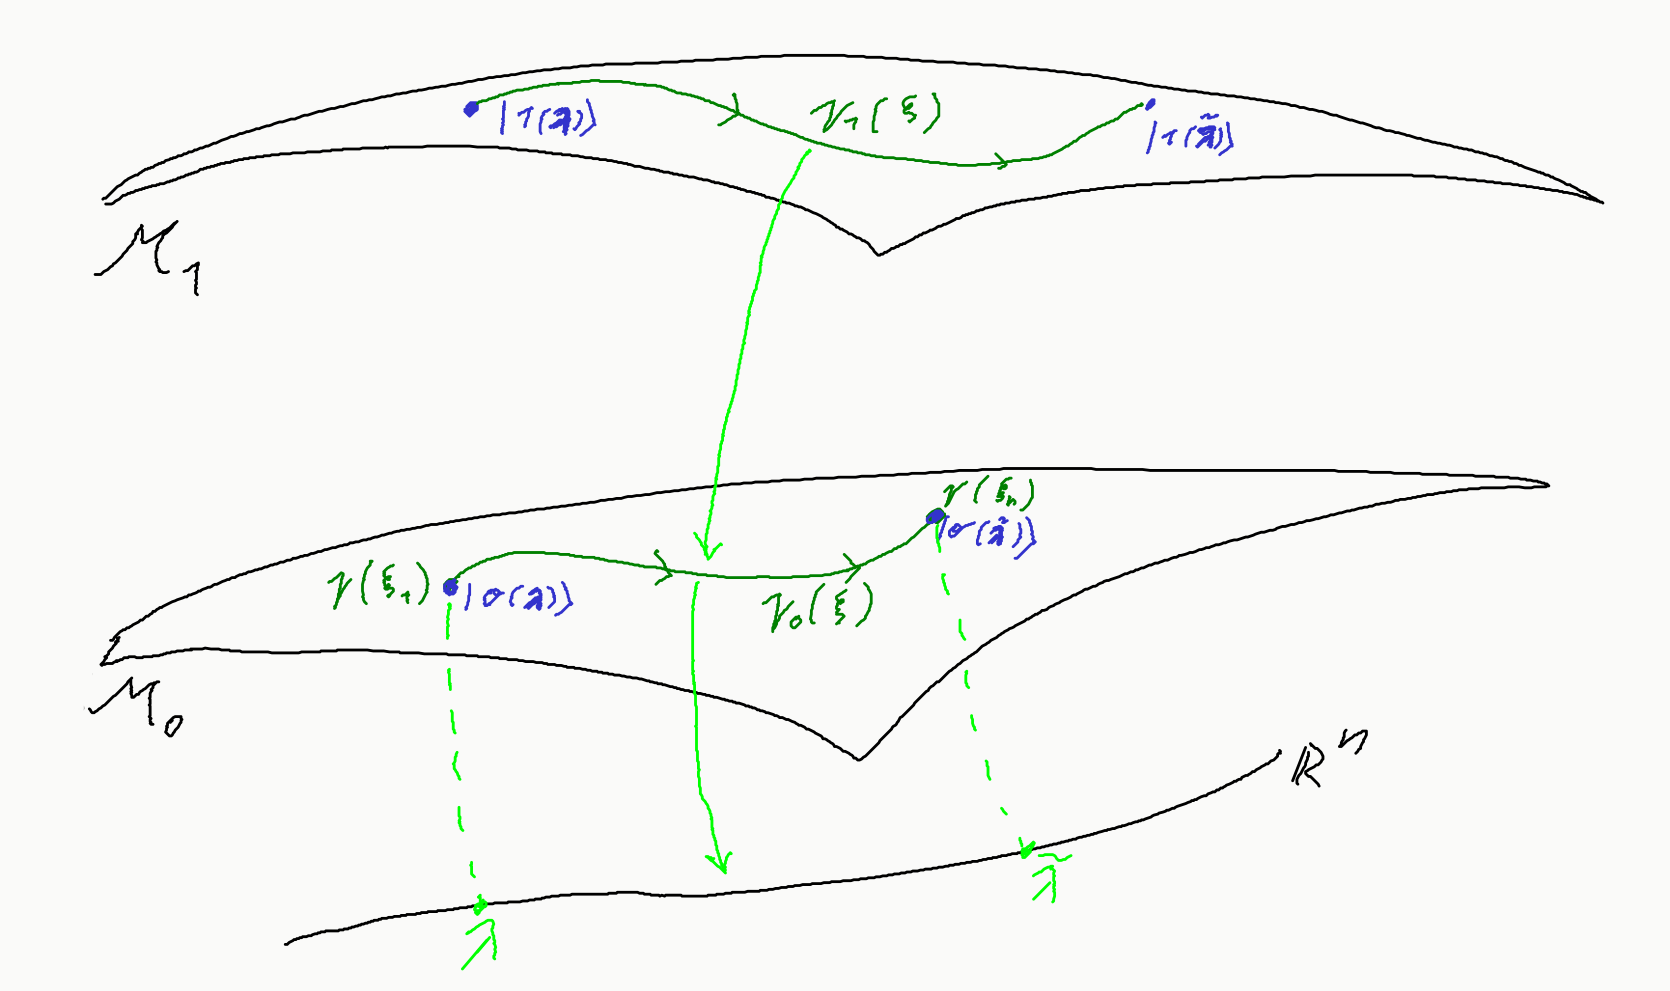
\includegraphics[width=\textwidth]{../img/manifoldCutIntuition.png}
\caption{Geometrical intuition for the \bluee{state} transport on fiber manifold sections $\M_s$ along the \greenn{curves}.\red{change $\xi$ to $t$ and states at point $\gamma(0)$ and $\gamma(T)$}\red{draw it as slices from the pictures above}}
    \label{fig:manifoldCutIntuition}
\end{figure}

Changing the state from eigenstate $\ket{s(\llambda)}\in\M_s$ to $\ket{s(\tilde\llambda)}\in\M_s$ during some time period is unitary transformation and can be thought of as \emph{parallel transport on fiber bundle} between two states. Assuming the transport goes along curve parametrized by time $\gamma_s(T)\coloneqq\{\llambda(t)|t\in(0,T)\}\subset \mathcal U$. The transported state can be written at any time as
\begin{equation}
    \hspace{-5pt}\ket{s(\llambda(t))} = \Par_{\gamma_s(t)}\ket{s(\llambda(0))} = \exp\left(-i\int_0^tE_s(\tau)\d\tau)\right)\exp(i\gamma_s(t))\ket{s(\llambda(0))}.
    \label{eq:phasesOnManifold}
\end{equation}
Let's describe the meaning of two exponentials in this transport.
\subsubsection{Dynamical phase}
The first exponential in Eq. \ref{eq:phasesOnManifold}, the \emph{dynamical phase}, is well known solution to the energy Schr\"odinger equation \ref{eq:energySchrodinger} and depends only on time and energy spectrum during the transport. This dynamical phase changes the states only within the projective state manifold $\P\M_s$. 

\subsubsection{Geometrical phase}
The complication arises with the fact that our playground is a state manifold $\M_s$ and some element $e^{i\varphi}=e^{i\gamma_s(t)}$, called \emph{geometrical phase} needs to be included. This phase is generally non-integrable, meaning it depends on the whole path and cannot be written simply as $\gamma_s(\llambda)$. For some closed curve on
\begin{equation}
    C=\{\llambda(t)|t\in[0,T] \text{, such that }\llambda(0)=\llambda(T)\}\subset \mathcal U
\end{equation} 
we generally get $\Par_C \ket{\psi(\llambda)}\neq \ket{\psi(\llambda)}$. This property is sometimes called an \emph{anholonomy} % and should be defined properly.
% \begin{definition}[Anholonomy]
%     Geometrical phenomenon, which causes some variable $V(\gamma(p))$ not to return to it's original value while varying it's parameter $p$ around some closed curve $\gamma(p)$. 
% \end{definition}
and geometric intuition can be seen on Fig. \ref{fig:parallelTransportClosed}. 
\begin{figure}[h]
    \centering
    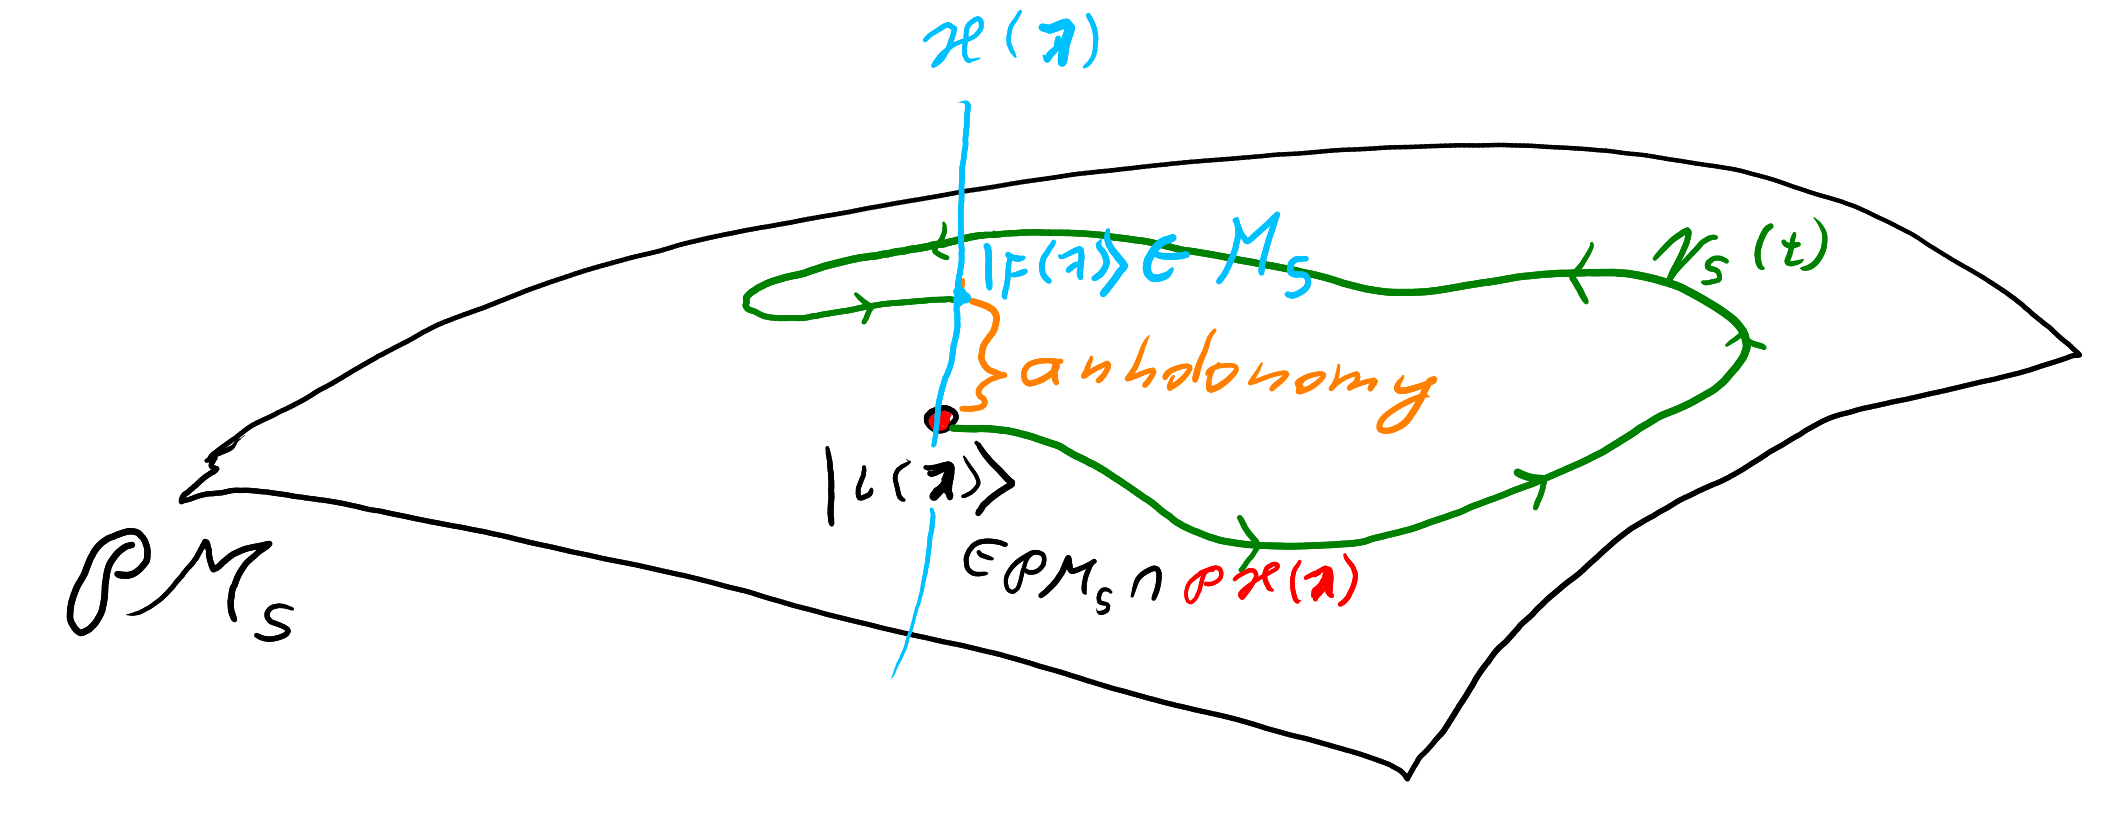
\includegraphics[width=0.8\textwidth]{../img/parallelTransportClosedCurve_1.png}
\caption{Parallel transport around some \greenn{closed curve $C$}. The \red{eigenstate $\ket{i(\gamma(0))}\in\P\M_s$} can be transported to another eigenstate $\ket{f(\gamma(T))}\in\M_s$. The \textcolor{orange}{anholonomy} represents their difference in a \blue{gauge} direction.\red{ressemble the pictures above, change the states to $\gamma(0),\gamma(T)$}}
    \label{fig:parallelTransportClosed}
\end{figure}

% For quantum states, the anholonomy can be measured as a non-zero angle between $\ket{V}$ and $\Par_C\ket{V}$, meaning
% \begin{equation}
%     \braket{V|\Par_C|V}\neq 0.
% \end{equation} 


Substituting general solution \ref{eq:phasesOnManifold} to Eq. \ref{eq:schrodinger} yields\footnote{Here the derivation along upper bound $F(x)\coloneqq\int_0^{g(x)}f(t)\d t \Rightarrow F'(x)=f(g(x))g'(x)$ for $f(t)\in L^1(0,g(x))$ and differentiable function $g$, is used.} 
\begin{align}
    \HH(\llambda(t))\kpsit &= i\der{}{t}\kpsit\\
    E_s(\llambda(t)) \ket{s(\llambda(t))} &= E_s(\llambda(t))\ket{s(\llambda(t))} -\der{\gamma(t)}{t}\ket{s(\llambda(t))}+ \der{}{t}\ket{s(\llambda(t))}\\
    \der{\gamma(t)}{t}&=i\braket{s(\llambda(t))|
    \der{}{t}|s(\llambda(t))}.
\end{align}
 Separating the dependence of vectors on driving parameter and time, we get
\begin{equation}
    \der{\gamma(\llambda(t))}{t} =i\braket{s(\llambda(t))|\partial_j s(\llambda)} \der{\llambda^j(\lambda)}{t} .
\end{equation}
Integrating this equation around some closed curve $C$ and assuming the dynamical phase to be zero, we get
\begin{equation}
    \gamma_s(C)=i\oint_C\braket{s(\llambda)|\partial_j s(\llambda)}\d \llambda^j.
    \label{eq:gammaCoint}
\end{equation}
We see, that the geometric phase does not depend on energy or time, only on the sequence of Hamiltonians, which means it depends only on the path itself.



\subsubsection{Restriction to 3-dimensional parametric space}
The problem of calculating Eq. \ref{eq:gammaCoint} lies in the element $\partial_\llambda s(\llambda)$, which locally requires knowledge of single-valued basis $\{\ket{0},\dots, \ket{n}\}$. This can be avoided in 3-dimensions using Stokes's theorem for $S$ as the surface with boundary $\partial S=C$, for coordinate gradient $\bm \nabla$
\begin{equation}
    \begin{split}
        \gamma_s(C) &= -\Im \iint_C \bm\d S \cdot \bm \nabla \times \braket{s(\llambda)|\bm \nabla n(\llambda)}\\
         &= -\Im \iint_C \bm\d S \cdot \braket{\bm \nabla s(\llambda)|\times|\bm \nabla s(\llambda)}\\
        &= -\Im \iint_C \bm\d S \cdot \sum_{m\neq s} \braket{\bm \nabla s(\llambda)|m(\llambda)}\times \braket{m(\llambda)|\bm \nabla s(\llambda)}\\
        &= -\iint_C \bm\d S \cdot \bm V_s(\llambda),
    \end{split}
    \label{eq:stokes}
\end{equation}
for 
\begin{equation}
    \bm V_s(\llambda) = \sum_{m\neq s} \Im \frac{
            \braket{s(\llambda)\bm \nabla_\llambda \HH(\llambda) |m(\llambda)}\times \braket{m(\llambda)|\bm \nabla_\llambda \HH(\llambda)|s(\llambda)}    
             }{
(E_m(\llambda)-E_s(\llambda))^2
             }.
\end{equation}
The element of summation $m=s$ in third step of derivation \ref{eq:stokes} is real, therefore has no influence on $\gamma_s$ and can be omitted. 

\begin{proof}
 All steps in Eq. \ref{eq:stokes} are simple algebraic operations, except for the last equivalence. This can be shown by differentiating the Schr\"odinger equation \ref{eq:energySchrodinger}. For any $\ket{s(\llambda)}\in \M_m,\;\ket{m(\llambda)}\in \M_m$ (the dependence on $\llambda$ in notation will be omitted), we get
\begin{equation}
    \begin{split}
        \bm \nabla (\overbrace{\HH(\llambda)\ket{s}}^{E_s(\llambda)\ket{s}})&= (\bm\nabla \HH(\llambda))\ket{\bm \nabla s} +\HH(\llambda) \ket{\bm \nabla s}\\
        \braket{m|E_s(\llambda)|s}&= \braket{m|\bm \nabla \HH(\llambda)| s}+ \underbrace{\bra{m} \HH(\llambda)}_{\bra{m} E_m(\llambda)} |\bm\nabla s\rangle \\
        \braket{m|\bm \nabla s}&=
        \frac{\braket{m|\bm \nabla \HH(\llambda) |s}}
        { E_s(\llambda)-E_m(\llambda)}, \qquad s\neq m,
    \end{split}
    \label{eq:mgradn_proof}
\end{equation}

where we used $\ket{\bm \nabla s}\coloneqq\bm \nabla \ket{ s}$.    
\end{proof} 

Comparing the first expression in Eq. \ref{eq:stokes} with its last one and extending it to real numbers, we get
\begin{equation}
    \bm V_s(\llambda)=\bm \nabla\times\braket{s(\llambda)|\bm \nabla m(\llambda)}, 
    \label{eq:vectorPotentialDef}  
\end{equation}
defining \emph{vector potential} $\bm V_s(\llambda)$.

As was mentioned, the above procedure from Eq. \ref{eq:gammaCoint} was performed only for three-dimensional space. Proper generalization to k-dimensional space would yield
\begin{equation}
    \gamma_s(C) = -\iint_C (\bm\d S)^{\alpha\beta} \cdot\Im \frac{
        \overbrace{\braket{s(\llambda)\bm\d_\alpha \HH(\llambda) |m(\llambda)}}^{\in\TT_1\M}\wedge \overbrace{\braket{m(\llambda)|\bm\d_\beta\HH(\llambda)|s(\llambda)}}^{\in\TT_1\M}    
    }{
        (E_m(\llambda)-E_s(\llambda))^2
    }.
    \label{eq:mgrads}
\end{equation}
                
                
                



\section{Fidelity}
The \emph{fidelity} measures "closeness" of two quantum states. It is generally defined for two density operators $\hat\rho, \hat\sigma$ as
\begin{equation}
    \begin{split}
        \mathcal F&: \End(\H)\times \End(\H)\mapsto \R, \\
        &\mathcal F(\hat\rho,\hat\sigma)\coloneqq \left(\Tr \sqrt{\sqrt{\rho}\sigma\sqrt{\rho}}\right)^2 = \left(\Tr\sqrt[4]{\rho \sigma \sigma \rho}\right)^2= \left(\Tr\sqrt[4]{\rho \sigma (\rho\sigma)^+ }\right)^2,
    \end{split}
    \label{eq:fidelitydef}
\end{equation}
where last term comes from hermiticity of density matrices.
The usefulness of this definition can be shown in three special cases.

\begin{itemize}
    \item If both states are pure, $\hat\rho\eqqcolon\ket{\rho}\!\!\bra{\rho}$, $\hat\sigma\eqqcolon\ket{\sigma}\!\!\bra{\sigma}$, the fidelity formula reduces to
    \begin{equation}
        \begin{split}    
            F: \H\times\H&\mapsto \R, \\
            \mathcal F(\hat\rho,\hat\sigma)  \equiv F(\ket{\rho},\ket{\sigma}) &= \left| \braket{\rho|\sigma}\right|^2.
        \end{split}
    \end{equation}

    \item If $\hat\rho=\ket{\rho}\!\!\bra{\rho}$ is a pure state, we have
    \begin{equation}
        \begin{split}
            \hspace{-23pt}\mathcal F(\ket{\rho}\!\!\bra{\rho},\hat\sigma) &= \left(\Tr\sqrt{\ket{\rho}\!\!\bra{\rho}\hat\sigma \ket{\rho}\!\!\bra{\rho}} \right)^2 = \bra{\rho}\hat\sigma \ket{\rho} \left(\Tr\sqrt{\ket{\rho}\!\!\bra{\rho}} \right)^2 = \bra{\rho}\hat\sigma \ket{\rho}
        \end{split}
    \end{equation}
    
    \item Commuting density matrices have a meaning of probability distributions. The commutativity implies that $\hat\rho,\hat\sigma$ can be diagonalized in the same eigenbasis. For $\hat\rho = \sum_i p_i \ket{i}\!\!\bra{i}$, $\hat\sigma = \sum_i s_i \ket{i}\!\!\bra{i}$ we get
    \begin{equation}
        \sqrt{\hat\rho \hat\sigma}=\Tr\left(\sum_k\sqrt{p_k s_k}\ket{i}\!\!\bra{i}\right)=\sum_k\sqrt{p_k s_k}
    \end{equation}
    and inserting into the definition \ref{eq:fidelitydef} gives
    \begin{equation}
        F(\hat\rho,\hat\sigma)=\left(\sum_k\sqrt{p_k s_k}\right)^2.
    \end{equation} 

\end{itemize}
    
    
The physical meaning of fidelity can be also seen on the state manifolds, imagining \emph{quantum quench between two states} (rapid change of some Hamiltonian parameters). In this case $F$ is the probability that system prepared in some initial ground state $\ket{\rho}$, is found in the new ground state $\ket{\sigma}$. $1-F$ is then the probability of exciting the system during this quench.

Before moving to the practical usage of fidelity, let's look at some general properties.
    

\begin{thm}[The fidelity properties]
    For any two density matrices $\hat\rho,\;\hat\sigma$
    \begin{itemize}
        \item $\mathcal F(\hat\rho,\hat\sigma)\in[0,1]$ (normalization),
        \item $\mathcal F(\hat\rho,\hat\sigma) = \mathcal F(\hat\sigma,\hat\rho)$ (symmetry),
        \item $\mathcal F(\hat\rho,\hat\sigma)=1 \Leftrightarrow \hat\rho\hat\sigma$.
    \end{itemize}
\end{thm}
\begin{proof}
    First statement is a consequence of Cauchy-Schwarz inequality. Second and third goes from Uhlmann's theorem, see for example \cite{uhlman}.
\end{proof}



\section{Metric and geometric tensor}
\label{chap:metricTensor}
As a playground for this chapter, we will choose the projective ground state manifold $\P\M_0\equiv \cup_{\llambda\in\R^d} \{\ket{o(\llambda)}\}$, but it can be easily generalized to any projective state manifold $\P\M_s$. This means the geometrical phase will be neglected, because the states are considered to be the physical states from the projective Hilbert space.
% Our first guess might be
% \begin{equation}
%     \d \tilde{s}^2 = \braket{i(\bm\llambda+\d\bm\llambda)|i(\bm\llambda+\d\bm\llambda)} = 1-2\Re{\braket{i(\bm\llambda+\bm\d\llambda)|i(\bm\llambda)}}.
% \end{equation}
% This is \emph{gauge dependent}, meaning that it depends on our choice of the wave phase, i.e. on observer. 

Let's first look at $\P\M_0$, which is needed to be \emph{gauge independent} in a sense, that the change in phase factor $\varphi(\lambda)$ of ground state $\ket{o(\llambda)}$ of the Hamiltonian $\HH(\llambda)$\footnote{Note that we can also write $\ket{o(\llambda)}\in \P\M_0\cap \H(\llambda)$, which is the set containing exactly one vector -- the ground state of $\HH(\llambda)$.}
\begin{equation}
    \ket{o(\llambda)}\mapsto e^{i\varphi(\llambda)} \ket{o(\llambda)}
\end{equation}
 induces the change 
\begin{equation}
        \braket{o(\llambda)|\bm \nabla o(\llambda)}\mapsto \braket{o(\llambda)|\bm \nabla o(\llambda)} + i\bm \nabla \varphi(\llambda) 
\end{equation} 
For $\varphi(\llambda)\in \mathcal C^2$, the gauge independent choice of phase $\phi$ would be for infinitesimal change for example
\begin{equation}
    f\coloneqq \braket{o(\bm\llambda+\delta\bm\llambda)|o(\bm\llambda)},
    \label{eq:fidelityDefinition}
\end{equation}
sometimes referred to as the \emph{fidelity amplitude of a ground state}, because for pure states we get the fidelity $F=|f|^2$. The meaning of fidelity as a probability transition between the states during some quench, leads to the definition of \emph{distance on $\M_0$}
\begin{equation}
    \d s^2 \equiv 1-F(\ket{o(\bm\llambda+\delta\bm\llambda)},\ket{o(\llambda)})= 1-\left|\braket{o(\bm\llambda+\delta\bm\llambda)|o(\bm\llambda)}\right|^2.
    \label{eq:distanceOnM0}
\end{equation}
We can easily check, that the axioms for metric distance holds:
\begin{itemize}
    \item identity of indiscernibles $s(\kpsi,e^{i\alpha}\kpsi) = 0 \Leftrightarrow \kpsi=\kphi$, $\alpha\in\R$,
    \item symmetry for any two states $\kpsi$, $\kphi$ is implied by $|\braket{\psi|\varphi}|=|\braket{\varphi|\psi}|$
    \item triangle inequality: $s(\kpsi,\ket{\psi_2}) <s(\kpsi,\ket{\psi_1}) + s(\ket{\psi_1},\ket{\psi_2})$ for any $\ket{\psi_1}$.
\end{itemize}
If we take the fidelity between two parameter dependent states, the infidelity $1-F(\ket{\psi(\llambda)},\ket{\psi(\llambda+\Delta)})>0$ and the first term of Taylor expansion in $\Delta$ is zero, implying it can be used for the metric tensor definition.

\begin{definition}[Metric tensor on projective state manifolds]
Because the projective state manifolds $\P\M_s$ are isomorphic to the base manifold $\R^n$, we can define
    \begin{equation}
        \begin{split}
            g_{\mu\nu}&: \T\mathcal U\times \T\mathcal U\rightarrow \R \\
            g_{jk}\d \bm \lambda^j \d\bm \lambda^k+\O(\lambda^3) \equiv \d s^2 &\coloneqq 1-\left|\braket{o(\bm\llambda+\delta\bm\llambda)|o(\bm\llambda)}\right|^2.
            \label{eq:metricTensorDef}
        \end{split}
    \end{equation} 
   
\end{definition}
Even though we call $g_{\mu\nu}$ the metric tensor \emph{on projective state manifolds}, it takes forms from $\T\mathcal U$. Using abstract indices this means
\begin{equation}
    g^{\mu\nu}\d_\mu \llambda \d_\nu \llambda.
\end{equation}
This whole procedure can be made more rigorous using so-called \emph{vector bundles}, see \cite{lu}[Chap. 7]. In our case we can use the bijection $\redd{\T\mathcal U}\times \redd{\T\mathcal U} \rightarrow \bluee{\T\M}\times \bluee{\T\M}$ and simply write
\begin{equation}
    g_{jk}\redd{\d\llambda^j \d\llambda^k} = g_{jk}\frac{\redd{\d\llambda^j}}{\bluee{\d\bm v^l}}\frac{\redd{\d\llambda^k}}{\bluee{\d\bm v^m}} \bluee{\d\bm v^l \d \bm v^m} \eqqcolon G_{lm}\bluee{\d\bm v^l \d \bm v^m}.
\end{equation}
In calculations only $g_{jk}$ is used, thus what should have been called \emph{the metric tensor on state manifolds} $G_{\mu\nu}$ leaves forgotten. "And some things that should not have been forgotten were lost." \citep{lordOfTheRings}







\subsubsection{Complex tensor generalization}
The scalar product (braket) of two quantum states is a 2-form $\chi_{\mu\nu}: \H\times\H\rightarrow \C$ and can be decomposed to real and imaginary part as
\begin{equation}
    \braket{\psi_1|\psi_2}\equiv \chi(\psi_1,\psi_2)=g(\psi_1,\psi_2)-i\nu(\psi_1,\psi_2).
    \label{eq:quantumProd}
\end{equation}

From braket sesquilinearity goes that $g_{\mu\nu}$ is symmetric and $\nu_{\mu\nu}$ antisymmetric, thus they can be uniquely written into one 2-form $\chi_{\mu\nu}$, called the \emph{Fubini-Study metric} or the \emph{Geometric tensor}, with property
\begin{equation}
    g=\Re \chi ;\qquad \nu=\Im \chi.
\end{equation}
Here we call the $g$ a \emph{metric tensor} and $k$ the \emph{curvature tensor}, or \emph{Berry curvature}. 

The geometric tensor is sometimes defined directly on the ground state manifold $\M_0$ from the fact, that the metric tensor is an analytical real function of coordinates, and we can make an analytical continuation into complex numbers, as
\begin{equation}
    \chi_{jk}\coloneqq \braket{\partial_j o|\partial_k o}_c \equiv \braket{\partial_j o|\partial_k o} - \braket{\partial_j o|o}\braket{o|\partial_k o},
    \label{eq:geometricTensor}
\end{equation}
where shortened notation $\partial_k\coloneqq\pder{}{\lambda^k}$ was used. The subscript $c$ means \emph{connected} and is defined in the formula.

The metric tensor can then be expressed as
\begin{equation}
    g_{jk} = \frac{1}{2}(\chi_{jk}+\chi_{kj}) = \Re\braket{\partial_j o|\partial_k o}_c = \Re \sum_{o\neq s}\frac{\braket{o|\pder{\H}{\lambda^j}|s}\braket{s|\pder{\H}{\lambda^k}|o}}{(E_o-E_s)^2}.
    \label{eq:metrictensorREdefinition}
\end{equation}
The Berry curvature is
\begin{equation}
        \nu_{jk} = \frac{i}{2}(\chi_{jk}-\chi_{kj})= \frac{1}{2}\Im\braket{o|[\curlyleftarrow{\partial}_k,\partial_j]|o}_c = - \Im \sum_{o\neq s}\frac{\braket{o|\pder{\H}{\lambda^j}|s}\braket{s|\pder{\H}{\lambda^k}|o}}{(E_o-E_s)^2},
    \label{eq:geom.tensorREdefinition}
\end{equation}
where $\curlyleftarrow{\partial}_k$ affects the object on the left.

%taylor is wrong
% \begin{proof}[Proof for Geometric tensor expression] In one-dimensional case we get from eq. \ref{eq:fidelityDefinition} using Taylor expansion and shortened notation $o\coloneqq o(\lambda)$
%     \begin{equation}
%         f=1+\braket{\partial_\lambda o|o}\delta\lambda-\frac{1}{2}\braket{\partial_\lambda^2 o|o}\delta\lambda^2+\mathcal{O}(\lambda^3),
%     \end{equation}
%     which plugged into eq. \ref{eq:distanceOnM0} gives
%     \begin{equation}
%         \begin{split}
%             \d s^2&=1-\bar{f}f=\left[-\braket{o|\partial_\lambda o}\braket{\partial_\lambda o|o}+\frac{1}{2}\braket{\partial_\lambda^2 o|o}+\frac{1}{2}\braket{o|\partial_\lambda^2 o}\right]\delta \lambda^2.
%         \end{split}
%     \end{equation}
%     Generalizing for $\lambda\in \R^d$, we get\footnote{assuming Hermiticity of the derivative operator everywhere on the ground state manifold}
%     \begin{equation}
%         \d s^2=\left[-\braket{o|\partial_j o}\braket{\partial_k o|o}+\underbrace{\frac{1}{2}\braket{o|\partial_j \partial_k|o}+\frac{1}{2}\braket{o|\partial_k \partial_j| o}}_{\Re\braket{\partial_mu o|\partial_k o}}\right]\delta \lambda^j\delta \lambda^k.
%     \end{equation}
%     Because only symmetric part contributes in the sum in eq. \ref{eq:metricTensorDef}, this proves symmetric part of equation \ref{eq:geometricTensor} and shows, that some more general tensor (\emph{geometric tensor}) exists.
% \end{proof}



\begin{proof}[Proof of the  metric tensor definitions correspondence]\
    \label{sec:derivationOfGeometricTensor}

    To prove the correspondence of geometric tensor, defined by Eq. \ref{eq:geometricTensor}, to distance on $\M_0$ in Eq. \ref{eq:distanceOnM0}, we start with the state $\ket{o(\llambda)}\in \M_s\cap\H(\llambda)$, which is the ground state of $\HH(\llambda)$. Changing parameter $\llambda$ to $\llambda+\delta \llambda$ results in a state, which is a linear combination of eigenstates $\ket{s(\llambda+\delta \llambda)}\in \M_s\cap\H(\llambda+\delta \llambda)$ of $\HH(\llambda+\delta \llambda)$, meaning the state is no longer a ground state. Probability amplitude of going to any new eigenstate is
    \begin{equation}
        \begin{split}
            a_s&=\braket{s(\llambda+\delta\llambda)|o(\llambda)}\approx \delta\lambda^j\braket{\partial_j s(\llambda)|o(\llambda)} \\
            &= -\delta\lambda^j\braket{s(\llambda)|\partial_j|o(\llambda)}.
        \end{split}
    \end{equation}

    If we introduce the \emph{gauge potential}, aka the \emph {calibration potential}, as\footnote{In SI units, the gauge potential is $\AA_j\coloneqq i\hbar\partial_{j}$}
    \begin{equation}
        \AA_j\coloneqq i\partial_{j},
    \end{equation}
    the probability amplitude can be expressed as
    \begin{equation}
    a=i\braket{s(\llambda)|\AA_j |o(\llambda)}\delta\lambda^j,
    \label{eq:probabilityOfTransitionIsGauge}
    \end{equation}
    which has a meaning of gauge potential matrix elements. Probability of the excitation, i.e. the transition to any state $s>0$ from ground state is then (omitting the $\llambda$ dependence in notation)
    \begin{equation}
        \begin{split}
            \sum_{s\neq 0}|a_s|^2&=  \sum_{s\neq 0} \delta \lambda^j \delta \lambda^k\braket{o|\AA_j|s}\braket{s|\AA_k|o}+\O(|\delta \lambda^3|) \\
            &= \delta \lambda^j \delta \lambda^k\braket{o|\AA_j \AA_k|o}_c\eqqcolon \delta \lambda^j \delta \lambda^k\chi_{jk}+\O(|\delta \lambda^3|),
        \end{split}
    \end{equation}
    where last term defines the geometric tensor.
\end{proof}






To understand why the gauge potential generates some calibrational invariance, we will define the Berry connection.
\begin{definition}[Berry connection]    
    On the ground state manifold $\M_0$, the \emph{Berry connection} is defined as the mean value of gauge potential
    \begin{equation}
        A_j(\llambda)\coloneqq \braket{o(\llambda)|\AA_j|o(\llambda)}= -i \braket{o(\llambda)|\partial_j|o(\llambda)}= -i\der{\lambda^j}{x^i} \braket{o(\llambda)|\pder{}{\lambda^j}|o(\llambda)},
        \label{eq:berryConnection}
    \end{equation}
    which uses the decomposition of $\llambda$ to some orthogonal basis $\{x_i\}_{i=1}^n$ of the base manifold $\R^n$. 
\end{definition}
    

This empowers us to take derivatives in any direction and the expression for geometric tensor on $\M_0$
\begin{equation}
    \chi_{jk}(\llambda) = \partial_j A_k(\llambda)-\partial_k A_j(\llambda)
    \label{eq:geometricTensor}.
\end{equation}
This formula can be directly proven by comparing with \ref{eq:geometricTensor}. Here we see that the calibrational invariance is 
\begin{equation}
    A_j \mapsto A_j+\partial_j \alpha(\llambda),\qquad \alpha\in\mathcal C^2,
\end{equation}
meaning any twice differentiable function can be added to the gauge potential, leaving the geometric tensor unchanged.

\begin{definition}[Berry phase]
    
    The \emph{Berry phase}, as an integral of the Berry connection along some closed curve $\mathcal{C}$\footnote{
        The reasonability of this definition can be seen, if we assume the ground state of a free particle
        $\braket{\bm{x}|i(\llambda)}\equiv i(\bm{x},\llambda)= |i(\bm{x})|e^{i\varphi(\llambda)}$,
        then the Berry connection is
        \begin{equation}
            A_j=-\int \d \bm{x}|i(\bm{x},\llambda)|^2\partial_j \varphi(\llambda) = -\partial_j \varphi(\llambda)
        \end{equation} 
        and Berry phase
        \begin{equation}
            \varphi_B=\oint_\mathcal{C} \partial_j \varphi \d \lambda^j,
        \end{equation}
        which represents total phase accumulated by the wave function. It is really the analogy for Berry phase in classical mechanics, which for example in the case Foucault pendulum on one trip around the Sun makes $\varphi_B=2\pi$
        }

    \begin{equation}
        \varphi_B\coloneqq-\oint_\mathcal{C} A_j(\llambda)\d \lambda^j=\int_\mathcal{S} \chi_{jk}(\llambda)\d \lambda^j \wedge \d\lambda^k,
    \end{equation}
    where we used the Stokes theorem for some area $\mathcal{S}$ with boundary $\partial\mathcal{S}=\mathcal{C}$.    
    
\end{definition}

Berry phase is zero, when the curve does not go around some geometric tensor singularity. This can be formally written using the \emph{winding number}, which counts \emph{how many times the curve goes counterclockwise around some point of interest}. In our case the points of interest are singularities $a$, and we say:
$$\mathrm{Ind}_a \gamma(\lambda)=0 \Rightarrow \varphi_B=0.$$

Those singularities appear in the system due to energy spectrum degeneracies, in the case of ground state manifold, when $E_1-E_0=0$. These points are called \emph{diabolic}, because of the energy spectrum shape in the $(\lambda,\chi)$ parameter space.\footnote{https://en.wikipedia.org/wiki/Diabolo}




















